\chapter{Validation software}

It was important to validate the calculations done in this project continuously. As many of the calculations are not static, but because of inertial forces is was important visualize these changes as they were happening. It was decided that implementing this feature in GeoMod would be to time consuming because of it's size and complexity. 

It was therefore necessary to create a smaller program that would be able to do the calculations and visualize the results. That way, the algorithms could be validated and their practicality determined as fast as possible. This approach can be compared to rapid prototyping in traditional manufacturing, fail early to succeed sooner.


\section{Interface}

\todo[inline]{
\textbf{Todo}

- Decribe \figref{interface} and \figref{console}
}

\begin{figure}[h!]
    \centering
    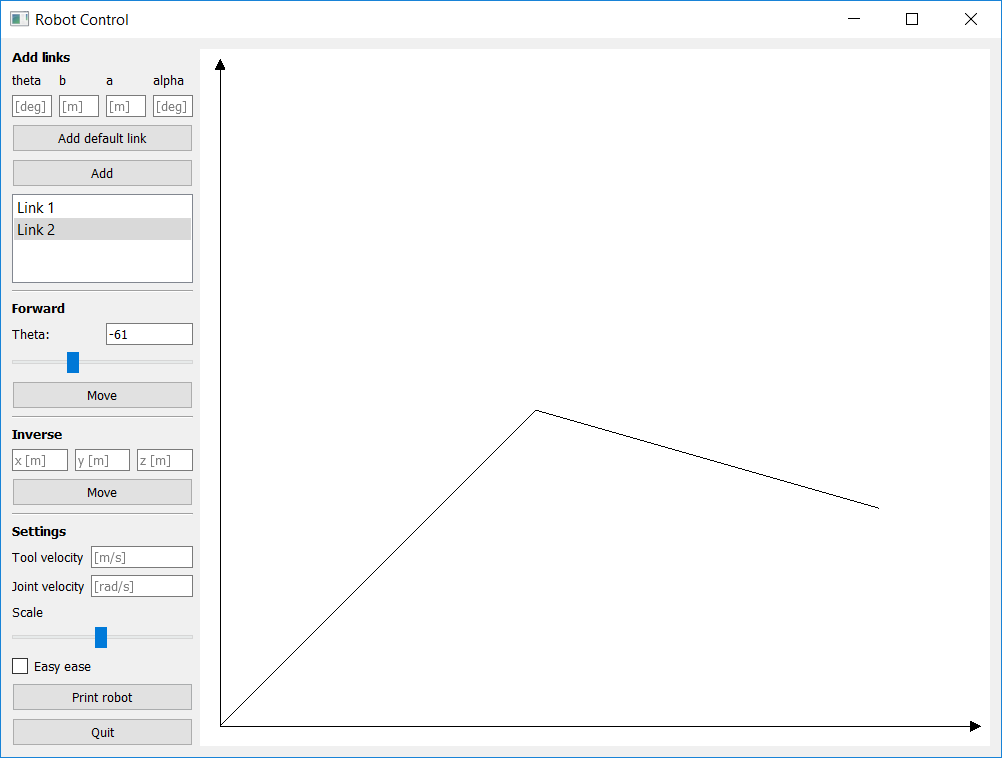
\includegraphics[width=.9\textwidth]{robot_control_interface}
    \caption{Main interface of \textit{Robot Control}, showing main drawing area and controls for adding links and moving them}
    \label{interface}
\end{figure}

\begin{figure}[h!]
    \centering
    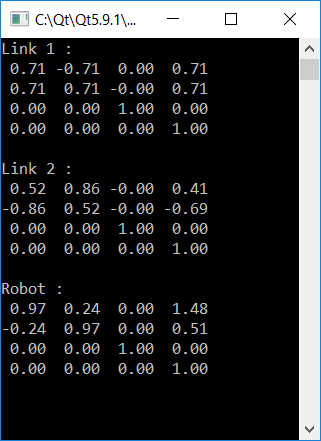
\includegraphics[width=.4\textwidth]{robot_control_console}
    \caption{Console was used to output transformation matrices and other useful information}
    \label{console}
\end{figure}

\section{Class overview}

\todo[inline]{
\textbf{Todo}

- Describe the intention and structure of the following classes:

- Robot, Link, Transformation and RenderArea class
}

\section{Drawing}

\todo[inline]{
\textbf{Todo}

- Describe how the QPainter class works

- Method for drawing arrows

- All the calculations are done for a 3D case, but everything is shown in 2D
}

\section{Animation}

\todo[inline]{
\textbf{Todo}

- It was important to have continuous moving links to verify the calculations

- start and end for each link can be set

- animation between these values, quintic graphs

- computer time is stored for last position so that derivatives can be calculated

- Must be calculated in a way that does not depend on the computer or available processing power, not a fixed frames per second
}